\subsection{News boy/vendor model}

We use the notation of Factory Physics (FP). Note that the formulas in
FP are in terms of integrals rather than with summations. We find this
unsatisfactory since it is easy to evaluate summations in excel (or an
other programming environment), and carrying out integration is often
much more difficult. For this reason we derive  results of FP in terms
of summations. 


We develop the newsvendor in stages.  Suppose that a shop sells some
perishable item with a life time of one day. It has to decide one day
ahead, or the morning before the shop opens, on the number of items to
order/make/prepare. The costs are
\begin{align*}
  p_b &= 5, \text{i.e., Buying price of one item} \\
  p_s &= 10,  \text{i.e., Selling  price of one item} \\
  p_e &= 3, \text{i.e, Salvage (end) value of one item} \\
  c_o &= \text{i.e., Overage cost, Cost of having  one  item over at the end of the day} \\
  c_s &= \text{i.e., Shortage cost, Cost of being   one  item short during the day} \\
\end{align*}
Cost for overage or underage are linear.  Let $X$ (a random variable)
be the number of units sold during a particular period, and let $Q$
denote the number of units ordered.  I assume that
$g_i = \P\{ X = i\}$ is given.


\begin{question}
  Can you express $c_o$ and $c_s$ in terms of the other cost parameters?
  \begin{solution}
    $c_o = p_b-p_e$ and $c_s = p_s-p_b$. 
  \end{solution}
\end{question}


\begin{question}
Suppose the daily demand is $X\in \{0,1\}$ and $g(0) = \P(X=0)=1/2 = g(1)$. What would be the best number of items $Q$ to make? 
\begin{solution}
  The profit of the choice $Q=0$ is 0. Now consider $Q=1$. What is the profit?  We pay for one unit, and sell it perhaps. If we don't sell it, we get the salvage value, if we sell it, we get the sales price. Thus, the profit is
  \begin{equation*}
    -p_b 1 + p_s\cdot 1/2 + p_e\cdot 1/2. 
  \end{equation*}
\end{solution}
\end{question}

\begin{question}
Suppose the daily demand is $X\in \{0,1\}$ and $g(0) = \P(X=0)=1/3 = 1- g(1)$. What would be the best number of items $Q$ to make? 
\begin{solution}
If $Q=1$ we make as a profit:
  \begin{equation*}
    -p_b 1 + p_s\cdot 2/3 + p_e\cdot 1/3 = -5 + 20/3 + 1> 0
  \end{equation*}
So, ordering $Q$ leads to a higher profit than ordering $Q=0$.
\end{solution}
\end{question}


\begin{question}
  What are the general terms that make up the profit function $Z(Q)$ if you were to order $Q$? 
  \begin{solution}
If you would order an amount $Q$, the profit consist of three terms: 
  \begin{itemize}
  \item expected number sold
  \item expected number left over
  \item order size
  \end{itemize}
  For the expected number of items sold, if the demand $X$ on a day
  turns out to be smaller than $Q$, we sell $X$; if $X>Q$ we only sell
  $Q$. Therefore, the expected sales is
  \begin{equation*}
    \E(\min\{Q,X\}). 
  \end{equation*}
The expected number of items over is $Q$ minus the expected sales: 
  \begin{equation*}
    Q-\E(\min\{Q,X\}) = 
    \E(Q-\min\{Q,X\})
  \end{equation*}
  where the second equation follows from the observation that the
  expected value of a constant is the constant itself, i.e.,
  $Q=\E(Q)$.  Thus, the total profit of buying $Q$ items must be
\begin{equation*}
Z(Q)=  -p_bQ+p_s\E(\min\{Q,X\}) + p_e\E(Q-\min\{Q,X\}).
\end{equation*}
  \end{solution}
\end{question}

\begin{question}
  Write $\E(X)$, i.e., the expected demand in terms of a summation.
  \begin{solution}
Recall that $\E(X)$ is just a short-hand for
    \begin{equation*}
      \E(X) = \sum_{i=0}^\infty i g(i).
    \end{equation*}
  \end{solution}
\end{question}

\begin{question}
  Can you write $\E(\min\{X,Q\}$ in terms of probabilities $g(i) = \P(X=i)$?
  \begin{solution}
From the previous question,
\begin{equation*}
  \E(\min\{(X,Q\})) = \sum_{i=0}^\infty \min(i,Q)g(i) = \sum_{i=0}^Q i g(i) + \sum_{i=Q+1}^\infty Q g(i).
\end{equation*}
Observe that $\sum_{i=Q+1}^\infty g(i)=\P(X\geq Q+1)$, thus we can simplify the above to
\begin{equation*}
  \E(\min\{(X,Q\})) = \sum_{i=0}^Q i g(i) + Q\P(X\geq Q+1).
\end{equation*}
  \end{solution}
\end{question}

\begin{question}
  Suppose for our example that the daily demand is $X\in \{0,1,2\}$
  and $g(0) = \P(X=0)=1/4$, $g(1)=1/3$, $g(2)=5/12$. What would be the
  best number of items $Q$ to make?
\begin{solution}
  Now we need to consider three different $Q$'s, $Q=0, 1,$ or $2$.
  Suppose that $Q=1$, then
\begin{equation*}
    \E(\min\{Q,X\}). =   \E(\min\{1,X\}). =   0\P(X=0) + 1\P(X=1)+1\P(X=2) = 1\cdot 1/3+1\cdot 5/12=9/12=3/4.
\end{equation*}
The expected number of items over is $Q$ minus the expected sales: 
  \begin{equation*}
    \E(Q-\min\{Q,X\}) = 1-3/4=1/4
  \end{equation*}
Thus,  for the example, the total profit is
\begin{equation*}
  -5\cdot1 + 10\cdot3/4+3\cdot1/4
\end{equation*}
is the expected profit per day of buying $Q=1$ at the start of the day. 

Once you implement this in excel, it is easy to experiment with
different values of $Q$ and see what is the best choice for $Q$. 
\end{solution}
\end{question}


\begin{question}
If the demand can be quite big, e.g., $X\in\{0,1,\ldots, 1000\}$, what is the slope of $Z(Q)$ for $Q$ small? What is the slope if $Q$ is big, i.e., near 1000? Assume that the demand distribution is something reasonable.
\begin{solution}
  If $Q=1$ it is very unlikely that the item will not be sold. In fact, we are nearly sure it will be sold, hence, the slope of $Z$ for small $Q$ must be $p_s$. If $Q$ is very large, we are pretty sure the `last item' will not be sold, hence, the slope must be $-p_e$. 
\end{solution}
\end{question}

\begin{question}
  Suppose there would be a setup cost which you have to pay to order any positive amount $Q>1$. What is then the profit? 
  \begin{solution}
    This is a no-brainer. If the setup cost is $s$, then just subtract
    $s$ from the profit function $Z(Q)$.
  \end{solution}
\end{question}

\begin{question}
Suppose we would set a certain service level, what is the profit under such a service level? Before we tackle this, what type of service level can we consider? 
\begin{solution}
  Cycle service level $P_1$, i.e., the probability that there are more
  items than demand, i.e., the fraction of periods/days that the shop
  does not run out of stock:
\begin{equation*}
P(X\leq Q) \geq P_1.
\end{equation*}

Another interesting service level is the fraction of demand that is met, i.e., the fill rate must be higher than some level $P_2$:
\begin{equation*}
\E(\min\{Q, X\})/ \E(X) \geq P_2
\end{equation*}
Realize that $\E(\min\{Q, X\})$ is the expected sales, while $\E(X)$ is the expected demand. The average amount of demand met is the sales divided by the demand.
\end{solution}
\end{question}

\begin{question}
  Now we can consider the profit under setting a certain performance level. How would you compute this?
  \begin{solution}
    If we want to focus on fill rate, first determine $Q$ such that
    $\E(\min\{Q, X\})/ \E(X) \geq P_2$, where $P_2=90\%$ or so. Call
    this $Q_2$. Then compute $Z(Q_2)$ to get the profit. 

    If we want to focus on cycle service level rate, first determine
    $Q$ such that $\P(X\leq Q) \geq P_1$, where $P_1=80\%$ or so. Call
    this quantity $Q_1$. Compute now $Z(Q_1$ to get the profit.
  \end{solution}
\end{question}

We next  discuss a few expressions that simplify the implementation of the profit function in excel.

\begin{question}
  Explain that $\E( \max\{Q-X, 0\})$ is another expression for the expected number of items over.
  \begin{solution}
    If $Q>X$, we have $Q-X$ over, if $Q\leq X$ we don't have items over. 
  \end{solution}
\end{question}

\begin{question}
  Write $\E (\max\{Q-X, 0\}) $ as a summation, so that you can implement this in excel.
  \begin{solution}
\begin{equation*}
  \begin{split}
  \E( \max\{Q-X, 0\} )
  &= \sum_{i=0}^\infty \max\{Q-i,0\}\P\{X=i\}\\
  &= \sum_{i=0}^\infty \max\{Q-i,0\}g_i\\
  &= \sum_{i=0}^Q (Q-i) g_i \\
  &= (Q-0) g_0 + (Q-1)g_1+ \cdots (Q-(Q-1))g_{Q-1} + (Q-Q)g_Q\\
  &= (Q-0) g_0 + (Q-1)g_1+ \cdots (Q-(Q-1))g_{Q-1} + 0 g_Q\\
  &= \sum_{i=0}^{Q-1} (Q-i) g_i.
  \end{split}
\end{equation*}
  \end{solution}
\end{question}


\begin{question}
  Why is $ \E( \max\{X-Q, 0\})$ the expected number of items short?
  \begin{solution}
    If there is a shortage of items, it must be that $X>Q$. The amount short is $X-Q$.
  \end{solution}
\end{question}

\begin{question}
  Write $\E (\max\{X-Q, 0\}) $ as a summation.
  \begin{solution}
\begin{equation*}
\begin{split}
     \E (\max\{X-Q, 0\} )
   &= \sum_{i=0}^\infty \max\{i-Q,0\}g_i\\
   &= \sum_{i=Q}^\infty (i-Q) g_i \\
   &= \sum_{i=Q+1}^\infty (i-Q) g_i.
\end{split}
\end{equation*}
\end{solution}
\end{question}


\begin{question}
  Let $Q=3$ and $g_1=g_2\ldots=g_5 = 1/5$. Compute $\theta = \E(X)$, i.e., the expected demand, the expected lost sales and the expected number over.
  \begin{solution}
    \begin{align*}
      \E( X) &= \sum_{i=1}^5 i g_i = 1/5+2/5+\cdots+5/5 = 3, \\
      \E (\max\{X-Q,0\}) &= \sum_{i=Q+1}^5 (i-Q) g_i = (4-3)/5 + (5-3)/5,\\
      \E (\max\{Q-X,0\}) &= \sum_{i=1}^{Q-1} (Q-i) g_i = (3-1)/5 + (3-2)/5.
    \end{align*}
  \end{solution}
\end{question}

\begin{question}
  Up to now we considered the profit function $Z(Q)$.  Can you
  establish a cost function of the newsvendor problem?
  \begin{solution}
The expected cost resulting from ordering an amount $Q$ follows
from combining the above formulas:
\begin{equation*}
     Y(Q) = c_o  \E( \max\{Q-X, 0\})  +   c_s \E( \max\{X-Q, 0\}) - c_s\E(X).
\end{equation*}
Note that the expected `cost' of selling $\E(X)$ of items should be subtracted from the cost. Since this term does not depend on the decision variable $Q$, it is often left out of the cost function, but formally it should be there.
  \end{solution}
\end{question}


\begin{question}
  Show that the profit is minus the the cost, i.e., $Z(Q) = -Y(Q)$.
  \begin{solution}
    Here we go:
    \begin{equation*}
      \begin{split}
        Z(Q) 
&=  -p_bQ+p_s\E(\min\{Q,X\}) + p_e\E(Q-\min\{Q,X\}) \\
&=  (p_e - p_b)Q+ p_s(\E(\min\{Q,X\}) - p_e\E(\min\{Q,X\}) \\
&=  (p_e - p_b)Q+ (p_s-p_e)(\E(\min\{Q,X\})\\
&=  -c_oQ+ (c_o+c_s)(\E(\min\{Q,X\})\\
&=  -c_o( Q - \E(\min\{Q,X\})) - c_s(\E(X) - \E(\min\{Q,X\}) + c_s\E(X)\\
&=  -c_o \E(Q-\min\{Q,X\}) - c_s\E(X-\min\{Q,X\}) + c_s\E(X)\\
&=  -c_o \E(\max\{Q-X,0\}) - c_s\E(\max\{X-Q,0\}) + c_s\E(X)\\
&=  -Y(Q).
      \end{split}
    \end{equation*}
Ensure you understand the last two steps. 
  \end{solution}
\end{question}

\begin{question}
Reproduce the results of the Christmas Lights Example of Factory Physics.
\begin{solution}
  First the data. We also use a library to handle the computations for
  the normal distribution. 


% \begin{minted}[mathescape, fontsize=\small, xleftmargin=0.5em]{python}
% from scipy.stats import norm
% c_o = 5 - 2.5
% c_s = 10 - 5
% mu = 10000
% sigma = 1000
% X = norm(loc=mu, scale=sigma) # demand
% \end{minted}


The result of the book is easy to produce. 


% \begin{minted}[fontsize=\footnotesize, xleftmargin=0.5em, mathescape]{python}
% >>> critical_fractile = c_s / (c_o + c_s)
% >>>
% >>> Q_star = X.ppf(critical_fractile)
% >>> Q_star
% 10430.727299295457

% \end{minted}

\end{solution}
\end{question}

\begin{question}
  In this christmas light example, 
do you think that $\sigma = 1000$ is reasonable? 
  \begin{solution}
    In all honesty, I think it is way too small. I would say that
    $\sigma=5000$ is much more reasonable. The problem is that if you
    would use this larger value, i.e., $\sigma=5000$, in the normal
    distribution, the probability that the demand is
    $\P(X<0)=\Phi((X-\mu)/\sigma < 0$ is not small anymore. However,
    the demand cannot be negative, hence using the normal distribution
    as an approximation of the demand is wrong for such cases. 

    Now this happens quite often: The problems in the books are tuned
    to showcase the simple methods developed in the book. However, as
    soon you have to do something real, the simple tricks all of a
    sudden don't work anymore. 
  \end{solution}
\end{question}


\begin{question} A Case to  Get rich in one day. 

  \begin{itemize}
  \item You plan to sell Napoleons tomorrow just outside of the
    Duisenberg building.
  \item How much money can you make? 
  \item How many Napoleons would you order today, to sell tomorrow?
  \end{itemize}
  Realize that this case contains a number of the problems related to
  dealing with perishable inventory, e.g., fashion. 

   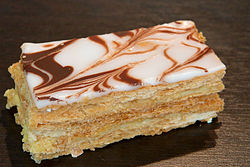
\includegraphics[scale = 1.0]{figures/mille-feuille}

   \begin{solution}
Here are the steps.
  \begin{itemize}
  \item Let's first assume that demand is normally distributed. Then
    we know from FP that $Q$ should be such that
    $G(Q) = c_s/(c_s+c_o)$.
  \item We make some assumptions about the prices. Take $p_s=0.75$,
    $p_b = 0.25$. $p_e=0$. Hence, $c_o = 0.25$, and $c_s = 0.5$.
  \item Thus, the critical fraction is $c_s/(c_s+c_o)=0.5/0.75 = 2/3$.
  \item Now compute $z$ with $\Phi(z)=2/3.$. Hence $z=0.43$.
  \item We also need some idea about the demand. How to get this?
  \item For Napoleons, we don't have yesterday's demand \ldots
  \item Can we use demand data of similar products?  I don't know what
    data to use. I have never tried to sell napoleons.
  \item Can we ask our sales force?  no. We don't have a sales force. 
  \item Last resort: make an educated guess; use powers of ten
    trick. Under this price model, I expect to sell more 1 napoleon,
    also more than 10, 100 might be, 1000 is too much. So, take
    $\mu=100$ as an estimate. Since I am not sure, $\sigma=30$ seems
    reasonable.
  \item If $\mu = 100$ and $\sigma = 30$, then $Q=0.43\sigma + \mu \approx 112$.
  \item Finally, what is the profit $Z(Q)$?
\item With the above formulas you can compute $Z(Q)$,  but let's use handwaving for a quick estimate. 
\item Note that $\min\{Q, X\} \leq X$, hence
  $\E \min\{X, Q\} \leq \E X= \mu$. If $\E \min\{X, Q\}\approx 95$,
  then $Z(112) \approx 95p_s - 100 p_b = 95\cdot 0.75 - 100 \cdot 0.25$.
  Since $95\approx100$, use this to simplify yet more:
  $Z(112) \approx 100(0.75-0.25) = 50$ Euro.
\item There are easier ways to make money!
  \end{itemize}
\end{solution}
\end{question}

\begin{question}
   Summarize the approach we took to some insight into this napoleon
   case, even though, initially, we had no idea about what profit we
   could make.
   \begin{solution}
Conclusion.
  \begin{itemize}
  \item Determine/estimate relation between demand (distribution) and sales price
  \item Make plots of the profit $Z$ as a function of $Q$, the demand
    distribution, and the sales price.
  \item Choose a $Q$ that makes sense. The existence of an optimal $Q$
    is a \emph{delusion}.
  \item Be aware that salesforce may predict too high demand. They get insentives to sell much, but they are not responsible for overage cost!
  \end{itemize}
   \end{solution}
 \end{question}


%%% Local Variables:
%%% mode: latex
%%% TeX-master: "notes_all"
%%% End:
